\subsubsection{Demoras de arribos y Cancelaciones}

Otro eje interesante es el de usar la cantidad de cancelaciones como
KPI. Se hipotetizó una relación dinámica entre las demoras y las
cancelaciones, ya que ambas pueden influirse mutuamente.

Para el análisis se agregaron los datos de todo el dataset por día
obviandose los datos del 2001, que presentan características propias
por la situación política y de seguridad.

Se eliminaron del dataset todas las cancelaciones debidas a factores
climáticos y de razones de seguridad, para disminuir el peso de
factores ajenos a la calidad del servicio.

\begin{figure}[h]
  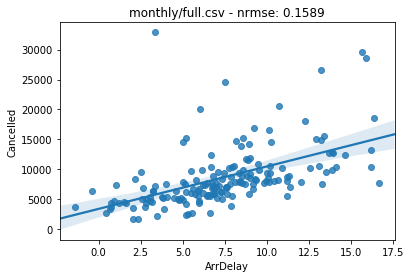
\includegraphics[width=0.6\textwidth, height=0.24\textheight]{./img/arrDel_vs_cancell.png}
  \centering
  \caption{ Relación entre las demoras de arribo y las cancelaciones,
    para todo el dataset desde 1994 hasta 2008 sin incluir 2001. Los
    datos están agregados por día. Las cancelaciones se sumaron, las
    demoras se promediaron.  }
  \label{fig:cancell-arrdelay}
\end{figure}

En la figura \ref{fig:cancell-arrdelay}, vemos una buena correlación
entre ambas variables con un \emph{nrmse} que si bien no es
despreciable, nos permite establecer una correlación lineal.

También nos preguntamos si las demoras o las cancelaciones, podían
afectar periodos posteriores. Para esto generamos una matriz de
correlación, para los mismos datos anteriores, tomando las
cancelaciones del día actual vs la demora y también las cancelaciones
de dos días en el futuro y en el pasado. En la figura
\ref{fig:cancell-arrdelay}. Se ve que la mayor correlación se
encuentran entre días concecutivos para las cancelaciones, incluso
superando la alta correlación entre demora y cancelaciones del día
actual mostradas en la fig. \ref{fig:cancell-arrdelay} \footnote{Las
  métricas no son iguales en ambas figuras.}

\begin{figure}[h]
  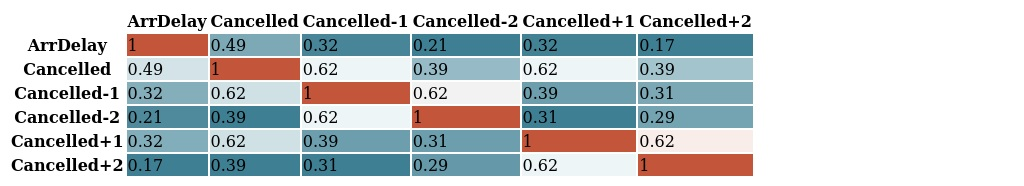
\includegraphics[width=0.6\textwidth, height=0.24\textheight]{./img/daily-full-csv-correlation-table.jpg}
  \centering
  \caption{ Correlacion entre las demoras de arribo y las
    cancelaciones para días cercanos. Las cancelaciones están
    shiteadas hacía adelante y hacía atrás. Los datos se tomaron para
    todo el dataset desde 1994 hasta 2008 sin incluir 2001. Los datos
    están agregados por día. Las cancelaciones se sumaron, las demoras
    se promediaron.  }
  \label{fig:cancell-arrdelay}
\end{figure}